\documentclass[12pt,a4paper]{article}
\usepackage[latin1]{inputenc}
\usepackage[english]{babel}
\usepackage{amsmath}
\usepackage{amsfonts}
\usepackage{amssymb}
\usepackage{graphicx}
\usepackage{array}
\usepackage{sidecap}
\usepackage{floatrow}
\usepackage{caption}
\usepackage{tabularx}

\author{Luis Vega - gutierre [at] rhrk.uni-kl.de \\ Pedro Torruella - torrue [at] rhrk.uni-kl.de}
\title{AXI4 - Stream interface}
\begin{document}
\vspace{-40mm}
\maketitle % Insert the title, author and date 
\vspace{-10mm}
\begin{center}
\includegraphics[scale=0.5]{images/ohne_titel.jpg}
\end{center}


\setlength\parindent{0pt} % Removes all indentation from paragraphs

\renewcommand{\labelenumi}{\alph{enumi}.} % Make numbering in the enumerate environment by letter rather than number (e.g. section 6)

\section{AXI4-Stream short introduction}

AXI4-Stream is an extension of the ARM-AMBA bus communication protocol intended to be used on streaming applications without dealing with complex control signals. Latest versions of Xilinx EDK (13 or higher) has built-in support for AXI4-Stream. Nevertheless, the documentation is very limited. That is why this short introduction could be a good starting point.

Basically, AXI4-Stream consists on a Master/Slave interface that can be employed for Writing/Reading respectively. The maximum number of Master/Slave interfaces on a Microblaze-based system is $16$ in total. Furthermore, AXI4-Stream is a $32$-bit bus communication protocol. Tables~\ref{t0a}, \ref{t0b}, \ref{t1a}, and~\ref{t1b} contain a brief description about the AXI4-Stream signals.


\begin{table}
    \begin{tabular}{ | c | c | c | c |}
    \hline
Signal & Direction & Width(bits) & Type \\ \hline
{\tt s\_axis\_tdata} & input & 32 &  data \\ \hline
{\tt s\_axis\_tvalid} & input & 1 & control  \\ \hline
{\tt s\_axis\_tlast} & input & 1 & control \\  \hline
{\tt s\_axis\_tready} & output & 1 & control \\ 
    \hline
    \end{tabular}
	\caption{AXI-Slave signals (details)}
    \label{t0a}
\end{table}

\begin{table}
    \begin{tabular}{ | c | c |}
    \hline
Signal & Description \\ \hline
{\tt s\_axis\_tdata} &  payload data \\ \hline
{\tt s\_axis\_tvalid} & receiving valid data, if s\_axis\_tvalid = '1'  \\ \hline
{\tt s\_axis\_tlast} & receiving last transaction value, if s\_axis\_tlast = '1' \\  \hline
{\tt s\_axis\_tready} & unit is ready to receive data, if s\_axis\_tready = '1' \\ 
    \hline
    \end{tabular}
	\caption{AXI-Slave signals (description)}
    \label{t0b}
\end{table}

\begin{table}
    \begin{tabular}{ | c | c | c | c |}
    \hline
Signal & Direction & Width(bits) & Type \\ \hline
{\tt m\_axis\_tdata} & output & 32 &  data \\ \hline
{\tt m\_axis\_tvalid} & output & 1 & control  \\ \hline
{\tt m\_axis\_tlast} & output & 1 & control \\  \hline
{\tt m\_axis\_tready} & input & 1 & control \\ 
    \hline
    \end{tabular}
	\caption{AXI-Master signals (details)}
    \label{t1a}
\end{table}

\begin{table}
    \begin{tabular}{ | c | c |}
    \hline
Signal & Description \\ \hline
{\tt m\_axis\_tdata} &  payload data \\ \hline
{\tt m\_axis\_tvalid} & sending valid data, if s\_axis\_tvalid = '1'  \\ \hline
{\tt m\_axis\_tlast} & sending last transaction value, if s\_axis\_tlast = '1' \\  \hline
{\tt m\_axis\_tready} & unit is ready to send data, if s\_axis\_tready = '1' \\ 
    \hline
    \end{tabular}
	\caption{AXI-Master signals (description)}
    \label{t1b}
\end{table}



\section{Why?}

AXI4-Stream is intended to be used on a MicroBlaze-Embedded-System, in order to send/receive data over an IP core. Therefore, the following system in figure~\ref{f0} will be used as reference  design for this documentation. Moreover, the main goal of this documentation is to provide essential knowledge to adapt or create IP-cores to work with AXI4-Stream in a MicroBlaze-Embedded-System. Additionally, extra functionality to the interface is added beside the communication interface itself. For example, a reset output that can be controlled by software. Thus, users could be able to reset their system easily. All these details will be covered in later sections.

\begin{figure}[!h]
\includegraphics[scale=0.35]{images/idea.png}
\caption{Microblaze Embedded System.}
\label{f0}
\end{figure}


\section{AXI-Slave interface}

\subsection{Brief description}

The AXI-Slave interface ({\tt AxiSlv.vhd}) is the module in charge of reading from the AXI4-Stream bus. Since the MicroBlaze can write into the AXI4-Stream bus, the AXI-Slave interface could be used to fetch data from MicroBlaze and send it to the IP of interest. The AXI-Slave block is shown in figure~\ref{f1}.

\begin{figure}[!h]

\includegraphics[scale=0.25]{images/axiSlvBlock.png}
\caption{AXI-Slave interface block}
\label{f1}
\end{figure}

The basic idea behind is a Serial-To-Parallel interface, data will come serially from ({\tt s\_axis\_tdata}) and then place it in register's array ({\tt reg\_array}). How the data are arranged in this register's array is shown in figure~\ref{f2}. The WIDTH and NUM\_REG variables are generic and let users configure the interface as it is needed. The WIDTH variable is used for assigning the data-width of ({\tt s\_axis\_tdata}). However, remember that AXI4-Stream work with $32$ bits, so this variable should be $32$. On the other hand, the NUM\_REG variable states the number of registers need by your application. For example, if your application needs to feed three $32$-bits-inputs, NUM\_REG should be $3$. These details will be covered in the following application example.

A valid signal {\tt reg\_array\_valid} is provided by the interface. This signal will stall at '1' when the interface has a first configuration valid. On the other hand, a reset output {\tt rst\_output} is given that can be controlled by software. Furthermore, supposed that you would like to test an {\it Adder} that has two inputs (number1, number2) and you want to reset this {\it Adder} before sending these numbers. Then, you need to send the data sequence (1, number1, number2) over {\tt s\_axis\_tdata}, where the first number in the sequence, '1' in this case, stands for activating this reset output. Otherwise, if you do not want to activate the {\tt rst\_output} the data sequence should be (0, number1, number2). Additionally to this, the number of cycles where the {\tt rst\_output} is activated can be configured by the variable NUM\_RST\_CYCLE in the {\tt AxiSlv.vhd} module. Moreover, the {\tt rst\_output} is activated after the data is written in {\tt reg\_array}. Finally, the reset can be active high or low by assigning '1' or '0' to G\_RESET\_ACTIVE variable.

\begin{figure}[!h]
\includegraphics[scale=0.5]{images/axiSlvReg.png}
\caption{AXI-Slave register organization}
\label{f2}
\end{figure}
 
\subsection{Application example}
In order to make clear the functionality of the AXI-Slave interface ({\tt AxiSlv.vhd}), an application example is given in this section. Indeed, the application example will focus on adapting a RNG module to work with AXI4-Stream and attaching it to a MicroBlaze. Therefore, it is possible to send/receive data from our computer to the RNG module. To achieve this, we need {\tt AxiSlv.vhd} (Interface) and {\tt RngUniformTausworthe88.vhd} (RNG) modules. This files are in the source repository.

First of all, a top module in VHDL is needed in order to connect the slave interface and the RNG. This top module should be as shown in the figure~\ref{f3}. We are going to call this module as {\tt AxiRng.vhd}. If you do not want to write the code, then look for the {\it AxiRng} folder in the source repository.

\begin{figure}[!h]

\includegraphics[scale=0.5]{images/axiRngBlock.png}
\caption{AxiRng.vhd}
\label{f3}
\end{figure}

The "AND-gate" is used here between {\tt rst\_output}, {\tt aresetn} and {\tt reg\_array\_valid} to perform the reset only when the interface loads a valid configuration or the system has been restarted at the begging. The {\tt reg\_arrray} signal contains the seeds to feed the RNG module. The RNG module will load these seeds after a reset is performed, then it will start to generate random numbers. Since the {\tt axis\_tlast} signal is not used, the signal is assigned to '0'. Last but not least, the generic values for the modules are:

\begin{itemize}
\item G\_RESET\_ACTIVE = 0
\item WIDTH = 32
\item NUM\_REG = 3
\item NUM\_RST\_CYCLE = 3
\end{itemize}

At this point, we can go further and follow some steps to see everything working. This documentation is based on Xilinx Design Suite 14.1 and a Virtex-6 ML605. Thus, it should be worth to check if you have both. All the steps are performed on the {\tt csiga} server, which has already installed all the necessary tools. The steps that you are going to perform on your host computer are in sections``Setting up the host" and ``Download HW/SW to the FPGA". For doing so, it is enough to have Xilinx Webpack 14.1, which is available and free on Xilinx website.

Because the development steps are based on different tools, it is suggested the folder tree structure shown in figure~\ref{f5}. After creating this structure, you should place the tree VHDL files in the ``vhdlSrc" folder:

\begin{itemize}
\item {\tt AxiRng.vhd}
\item {\tt AxiSlv.vhd} 
\item {\tt RngUniformTausworthe88.vhd}
\end{itemize}

The ``ise, xps and sdk" folders should be empty, because the project files are going to be saved there. Finally, the following steps are given in a {\it Quick start} fashion, if you are interested in more details, you can check other documentation about Xilinx Design Suite 14.1 that is available in the repository.

\begin{figure}[!h]
\includegraphics[scale=0.60]{images/folderTreeStructure.png}
\caption{Project folder tree structure}
\label{f5}
\end{figure}

\subsubsection{Building the IP core - ISE}
\begin{enumerate}
\item Open Xilinx-ISE.
\item Create a new project with the name ``AxiRng" and placed it in the suggested location (``ise" folder).
\item Select the target FPGA-board (Virtex-6 ML605 revision D).
\item Add the source files to the project, this can be done by the ``Add copy of source" option in ISE.
\item Select our top module "AxiRng.vhd" and synthesize it, check that there are not errors here.
\item Close ISE and follow the next section.
\end{enumerate}

\subsubsection{Hardware assembly - XPS}
\begin{enumerate}
\item Open Xilinx-XPS.
\item Create a new project and placed it in the suggested location (``xps" folder).
\item Select the target FPGA-board (Virtex-6 ML605 revision D).
\item Keep the RS232\_UART peripheral and remove the other peripherals. Remember to activate the interrupt in the check-box.
\item Click finish.
\item In this step, we are going to create a dummy peripheral in order to use it as template to build our MPD file, because the tool does not help us on that. Go to hardware and ``Create or Import Peripheral..", then name it ``template". Select AXI4-Stream bus interface and the number of input/output 32-bit words should be '1'.
\item Similarly, the AxiRng can be imported. In this case, instead on selecting create you should select ``import existing peripheral". Then, go to our ``ise" folder and find the ``AxiRng.prj" file. After this, use the same name ``AxiRng", so the tool can find the top module. The following configuration steps by the wizard should be avoided by unchecking the box.
\item Open the MPD file for the dummy peripheral, this can be done by going to the IP catalog and expanding USER and right click on ``template" , then click on ``View MPD". Copy everything down from ``\#\#BUS Interfaces" to the end of the file.
\item Open the MPD file for our AxiRng and paste it in the same lines from where you copied it in the other file. Then, make all the necessary modifications as shown in the figure~\ref{f6}.
\item Go to ``Project" and click on ``Rescan User Repositories". 
\item Now, after the peripheral description of the AxiRng is done, we can add it to the system assembly view by double clicking on it.
\item In order to make the connection between the AxiRng and the MicroBlaze, a AXI4-Stream bus has to be instantiated. This can be achieved by double clicking on microblaze\_0 in the assembly view. Then, click on next button until you reach ``PVR and Buses", find ``Select stream interfaces" and choose ``AXI" instead of ``FSL", and ``Number of stream links" should be '1'. Click ok.
\item Connect the AxiRng by clicking on the respective bus in the system assembly view. M0\_AXIS on microblaze\_0 should be connected to S0\_AXIS on AxiRng. The same for S0\_AXIS on microblaze\_0 should be connected to M0\_AXIS on AxiRng.
\item Afterwards, the clock and reset signal of the AxiRng must be connected. Go to the port tab in the system assembly view and look for AxiRng. Then, click on ACLK and select ``clock\_generator\_0" and select ``CLK0" in the right side. The reset can be connected in a similar way, find the ``ARESETN" port and click it. Then, select ``proc\_sys\_reset\_0" and ``Peripheral\_aresetn".
\item Now, the complete MicroBlaze Embedded System can be generated. This can be accomplished by clicking on `Export Design". Remember that you can speed up the process by going to edit $\rightarrow$ preferences and enable the ``Parallel synthesis" option. 
\item When the process finished, Xilinx-SDK should pop up and ask for a workspace folder. Please select the suggested folder (``sdk" folder). Xilinx-SDK will create a sub folder named ``hw\_platform", this folder contain the bitstream file (*.bit). Usually, this file is called ``system.bit". Later, this ``system.bit" will be used for programming the FPGA.
\end{enumerate}

\begin{figure}[!h]
\includegraphics[scale=0.75]{images/axiMpd.png}
\caption{AxiRng MPD file}
\label{f6}
\end{figure}

\subsubsection{Software development - SDK}
\begin{enumerate}
\item After selecting the workspace folder as you did in the last step, you should be able to see the eclipse environment. Check that the ``hw\_platform" folder created by XPS is placed in the project explorer window in Xilinx-SDK. 
\item Go to ``File" and create a new ``Xilinx C project".
\item Select the ``hello world" template. Xilinx-SDK will create two folders, one containing the source code and the other one containing drivers and support libraries. These two folders are: ``hello\_world\_0" and ``hello\_world\_bsp\_0". As stated before, the ``hello\_world\_0" folder contain the source code (*.c) in the ``src" folder and the executable (*.elf) in the ``Debug" folder. The following information goes for advanced users, the build-configuration should remain in Debug-mode since the MicroBlaze Debug Mode (MDM) is going to be used for programming and test our system.
\item Then, in the ``hello\_world.c" file copy the code shown in the figure~\ref{f7}. 
\item Now, after saving the file, the project should be built again. However, you could double check building it again.
\end{enumerate}

\begin{figure}[!h]
\includegraphics[scale=0.75]{images/axiRngSwCode.png}
\caption{Source code for testing AxiRng}
\label{f7}
\end{figure}

\subsubsection{Setting-up the host}
\begin{enumerate}
\item Find a terminal application in your host computer. For example hyperterminal (Win) or cutecom (Linux).
\item Configure such terminal application to work on $baud rate=9600$, $data bits=8$, and $stop bits=1$.
\item Start or Open the device in order to start receiving values right after the programming is done.
\end{enumerate}

\subsubsection{Download HW/SW to the FPGA}
\begin{enumerate}
\item Download the bitstream file (system.bit) and executable (hello\_world.elf) from the server to your host computer. Remember that these files are in the ``hw\_platform" and ``hello\_world\_0/Debug" subfolder in the ``sdk" folder respectively.
\item Move the files to a handy location in your host computer, for example, your home folder.
\item Open a terminal there and type XMD and press enter. You should now be in the MicroBlaze Debug Module.
\item Type ``fpga -f system.bit" and press enter, this will download the bitstream file to the FPGA.
\item Type ``connect mb mdm" and press enter, this will connect the MicroBlaze to the Debug Module.
\item Type ``dow hello\_world.elf" and press enter, this will download the executable to our system.
\item Type ``rst" and press enter, in order to reset the microblaze. 
\item Type ``con" and press enter, this will start the software program.
\item Then, you should receive the first ten random values as shown in figure~\ref{f8}.
\item You could stop the MicroBlaze by typing ``stop" in the XMD environment. Also, you can find more useful commands in the MicroBlaze documentation.
\item The following information is to speed-up the programming procedure. You could copy all these commands into a file and after initializing XMD, and then you can perform ``source myfile.txt".
\end{enumerate}

\begin{figure}[!h]
\includegraphics[scale=0.5]{images/rngVal.png}
\caption{First ten random values - AxiRng}
\label{f8}
\end{figure}

\section{AXI-Master interface}

The AXI-Master interface ({\tt AxiMst.vhd}) is the module in charge of writing to the AXI4-Stream bus. Since the MicroBlaze can read from the AXI4-Stream bus, the AXI-Master interface could be used to send data to the MicroBlaze from the IP-core of interest. The AXI-master block is shown in figure~\ref{f9}.

\begin{figure}[!h]
\includegraphics[scale=0.25]{images/axiMstBlock.png}
\caption{AXI-Master interface block}
\label{f9}
\end{figure}

Opposite to the AXI-Slave interface, the AXI-Master interface works as a Parallel-To-Serial interface. In other words, data will come in a parallel fashion through {\tt reg\_array} and place it serially over {\tt m\_axis\_tdata}. Loading the data in {\tt reg\_array} can be done by a valid signal called {\tt reg\_array\_valid}, and it must be set to '$1$' for data loading. In addition to a valid signal, a ready signal ({\tt reg\_array\_ready}) is used for stopping data loading when the interface is serializing and putting data on {\tt m\_axis\_tdata}. Furthermore, when ready signal is '$1$', the interface is ready for receiving data. Otherwise, the ready signal will be '$0$'.

How the data are arranged by the AXI-Master interface is shown in figure~\ref{f10}. Similar to the AXI-Slave interface, the WIDTH and NUM\_REG variables are generic and let users configure the interface as it is needed. Remember that AXI4-Stream work with $32$ bits, so WIDTH should be $32$. More details, will be covered by the application example in the next section.

\begin{figure}[!h]
\includegraphics[scale=0.5]{images/axiMstReg.png}
\caption{AXI-Master register organization}
\label{f10}
\end{figure}

\subsection{Application example}

In the following application example, we will use AXI-Slave ({\tt AxiSlv.vhd}) and AXI-Master ({\tt AxiMst.vhd}) interfaces together with two RNG modules working in parallel. At the end of this application you should be able to adapt your own IP-core to work with the above mentioned interfaces.

First of all, a top module in VHDL is needed in order to connect all blocks. This top module should be as shown in the figure~\ref{f11}.  We are going to call this module as {\tt AxiTwoRng.vhd}. If you do not want to write the code, then look for the {\it AxiTwoRng} folder in the source repository.

\begin{figure}[!h]

\includegraphics[scale=0.4]{images/axiTwoRngBlock.png}
\caption{AxiTwoRng.vhd}
\label{f11}
\end{figure}

Similarly to the application example of AXI-Slave, the RNG module is connected to the AXI-Slave. However, there are some additionally details. First, the {\tt reg\_array} signal will contain six seeds for the RNG modules, three seeds for each one. Secondly, the generic parameters for the {\tt AxiTwoRng.vhd} is used as follows:

\begin{itemize}
\item G\_RESET\_ACTIVE = 0
\item WIDTH = 32
\item NUM\_REG\_SLV = 6
\item NUM\_REG\_MST = 2
\item NUM\_RST\_CYCLE = 3
\end{itemize}

The number of registers (NUM\_REG\_SLV) is $6$, because as it is stated before we need six seeds. Here, it might be good to remember that the number of registers is named as NUM\_REG\_SLV and not as NUM\_REG. The main reason is that we need to make a difference between the number of registers for the Slave and Master interface. Therefore, the number of registers for the AXI-Master is given by NUM\_REG\_MST. Furthermore, since we are instantiating two RNG modules, the application will produce $64$ bits. Thus, the parameter NUM\_REG\_MST should be $2$. Finally, the number of clock cycles for the reset (NUM\_RST\_CYCLE) is $3$.

On the other hand, the AXI-Master can control the generation of random numbers by the {\tt reg\_array\_ready} signal. Meanwhile, each valid signal {\tt valid} of the RNG modules is connected through an AND gate to the {\tt reg\_array\_valid} port.

At this point, we should have the following source files:

\begin{itemize}
\item {\tt AxiTwoRng.vhd}
\item {\tt AxiSlv.vhd}
\item {\tt AxiMst.vhd} 
\item {\tt RngUniformTausworthe88.vhd}
\end{itemize}

From now on, it is advisable follow the same directions given by the application example for the AXI-Slave interface. However, here are some additional hints:

\begin{itemize}
\item The MPD file is the same used in the AxiRng application example, since the interface is the same.
\item The software program (.c) for the AxiTwoRng application example is shown in figure~\ref{f12}.
\item The output for this application example is shown in figure~\ref{f13}.
\end{itemize}

\begin{figure}[!h]
\includegraphics[scale=0.75]{images/axiTwoRngSwCode.png}
\caption{Source code for testing AxiTwoRng}
\label{f12}
\end{figure}

\begin{figure}[!h]
\includegraphics[scale=0.5]{images/twoRngVal.png}
\caption{First eight random values - AxiTwoRng}
\label{f13}
\end{figure}


\end{document}